\chapter{Asking Strangers How Much Money They Make}

This chapter is based on a School of Hard Knocks entrepreneurship interview in downtown Austin, curated by LazyingArt LLC through Video2Book. The spoken question is simple: what was the most money you ever made in a single year? The answer is not simple. Some people refuse to say. Some answer with a range. Some answer by explaining a business, a career path, a management principle, or a risk they took before the money appeared. We will treat the numbers as evidence, but the real object of study is the mechanism behind them: capital, ownership, relationships, risk, assets, and skill.

\section{The Question Money Makes People Answer Around}

The interview begins with a direct question:
\[
I_{\mathrm{year}} = \hbox{most money made in one year}.
\]
That is the nominal variable. But the early answers show that this variable is guarded. One person says he is not going to tell. Another says he does not want to disclose personal income. An entrepreneur answers, instead, that ``we spend money, we make money.'' The point is already visible: annual income is not a clean measurement unless we know what kind of machine produced it.

A useful notation for this chapter is:
\begin{equation}
I_{\mathrm{year}} \neq R \neq \Pi .
\end{equation}
Here \(I_{\mathrm{year}}\) is personal annual income, \(R\) is business revenue, and \(\Pi\) is profit. The transcript gives several income and revenue claims, but it does not give margins, taxes, ownership percentages, or distributions. We therefore keep the quantities separate.

The hosts also give their own context. They say that they started a channel at the University of Texas and grew it to \(1.4\) million followers. That number matters because it changes the status of the question. This is not a private survey. It is a public interview format built on repeated attempts, public curiosity, and the willingness to ask strangers questions that most people avoid.

\section{Funding Discipline Before Scaling}

The first substantial interviewee identifies his field as neurotechnology. He says he is in the business of getting people off psychiatric medication and using frequencies or digital frequency patterns to restore mental health or general health. Those claims should remain attributed to him. What is more directly useful for entrepreneurship is the advice that follows when he is asked what he would tell himself at the start of his first business.

His answer is financial caution. Do not borrow money, he says, and if you do borrow, be very careful. His strongest sentence is that the biggest mistake he made was letting banks lend him money. He recommends funding the business yourself as much as possible, raising from friends and family, or using available platforms.

We can write the financing choice as a simple ordering, not as a theorem:
\begin{equation}
\hbox{preferred early capital}
  \approx
  \hbox{self-funding}
  \rightarrow
  \hbox{friends/family}
  \rightarrow
  \hbox{platform funding}
  \rightarrow
  \hbox{bank debt with caution}.
\end{equation}
The arrow does not mean that bank debt is always wrong. It means that, in this speaker's experience, fixed obligations were dangerous enough to become the central regret.

\subsection{Question \& Answer}

\paragraph{Question.}
If capital helps a business grow, why warn against borrowing from banks?

\paragraph{Answer.}
Because borrowed capital is not just money. It is money plus an obligation. A young business has uncertain revenue; debt often has fixed repayment demands. The mismatch is the danger. In compact form,
\begin{equation}
\hbox{debt pressure}
  =
  \hbox{fixed payment}
  -
  \hbox{reliable surplus cash flow}.
\end{equation}
When reliable surplus cash flow is small or uncertain, the obligation can control the business. The speaker's warning is therefore not anti-growth. It is a warning about the timing and structure of growth capital.

\section{Vertical Managers, Horizontal Managers, And Listening}

The same interviewee then turns from funding to scaling. He says he is the CEO of a public company and runs his own business. His management distinction is vivid. There are vertical managers, who sit on top, bark, and give orders. Then there are horizontal managers, where people sit at the table and work together.

The important detail is that he does not eliminate authority. He says that only in a critical moment does he pull rank and make a final decision. The management rule is therefore not pure consensus. It is collaborative work with a reserved decision right.

\begin{figure}
\centering
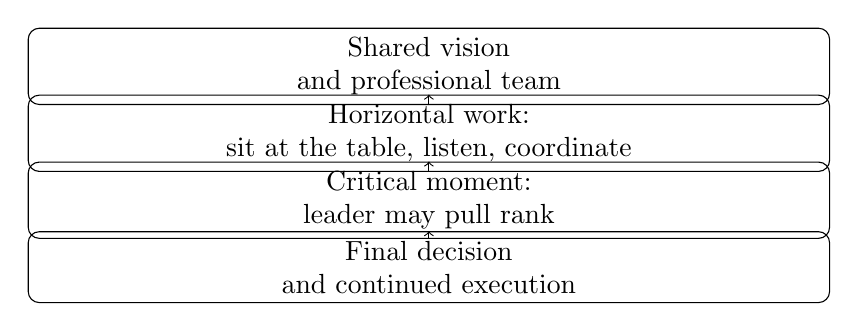
\begin{tikzpicture}[node distance=0.85cm]
\node[draw, rounded corners, align=center, text width=0.82\linewidth] (vision) {Shared vision\\and professional team};
\node[draw, rounded corners, align=center, text width=0.82\linewidth, below of=vision] (listen) {Horizontal work:\\sit at the table, listen, coordinate};
\node[draw, rounded corners, align=center, text width=0.82\linewidth, below of=listen] (critical) {Critical moment:\\leader may pull rank};
\node[draw, rounded corners, align=center, text width=0.82\linewidth, below of=critical] (decision) {Final decision\\and continued execution};
\draw[->] (vision) -- (listen);
\draw[->] (listen) -- (critical);
\draw[->] (critical) -- (decision);
\end{tikzpicture}
\caption{Transcript-backed management structure: collaboration is the default, decisive authority is reserved for critical moments.}
\end{figure}

The scale mechanism is social before it is numerical. Surround yourself with professionals or aspiring professionals, share the vision, and listen. He says people are too ready for a fight, and that posture should not be brought into a business.

\section{Relationships Are Access, Value Is Permission To Stay}

After a declined interview and a short behind-the-scenes sequence, the hosts describe their own operating method. They ask everywhere: at the mall, in line for food, outside ordinary shops. Their method is persistence under uncertainty. They are always, in their phrase, shooting their shot.

The next business thread comes from a VP of marketing at a software company. He says startups let him touch many different areas, while some colleagues became pigeonholed in one specific role. He says this let him grow faster than if he had taken a comfortable high-paying job at the beginning. The mechanism is breadth:
\begin{equation}
\hbox{learning rate}
  \uparrow
  \quad\hbox{when}\quad
  \hbox{role surface area}
  \uparrow .
\end{equation}
This is not a measured equation. It is the compact form of his career claim: more kinds of responsibility created more chances to learn.

When asked what matters more, what you know or who you know, he answers: who you know, one hundred percent. But the lecture does not stop there. The next speaker sharpens the point. Yes, it matters to surround yourself with millionaires, billionaires, and people ten steps ahead. But once inside those circles, you must provide value.

\subsection{Question \& Answer}

\paragraph{Question.}
Is success about who you know or what you can do?

\paragraph{Answer.}
The transcript resolves the tension by making the two variables sequential. Relationships may open the door; value keeps the door open. A useful working expression is:
\begin{equation}
\hbox{durable relationship}
  \approx
  \hbox{access}
  +
  \hbox{provided value}.
\end{equation}
Access without contribution becomes fragile. Skill without access can remain unseen. The interviewees treat the durable business relationship as the combination.

\section{Self-Employment, Risk, And The Market's Indifference}

The next medical-business owner refuses to disclose his exact income but answers that it was ``a lot.'' He says he has been in medical for \(26\) years and has owned his own business. Then he gives a harder lesson: working for yourself is not for everybody.

His concrete claim is that he has owned a stem cell company for \(17\) years and has a business doing more than \(4\) million in revenue. We preserve the claim as revenue:
\begin{equation}
R > \$4{,}000{,}000.
\end{equation}
We should not rewrite this as personal income or profit. Revenue is top-line business activity; it does not tell us margins, debt, payroll, tax, or owner distribution.

His advice is competitive. Take chances. After the first year, he says, nobody cares where you went to school. The market becomes ``you versus the rest of the world.'' His father gave him two pieces of advice: people buy from people they like, and one should control the controllables. The first is a sales mechanism, not just a slogan. If trust lowers friction, then likability and reliability become commercial assets. The second is an attention rule: spend scarce energy where action can change the result.

\section{Assets, Liquidity, And Strategic Timing}

The next major shift is from income to assets. A former military professional says that while moving through duty stations he bought houses, rented them out, and gradually became an investor without fully realizing it. By the time of the interview, he says:
\begin{equation}
N_{\mathrm{properties}} = 4.
\end{equation}
He also says he is cash poor and asset rich. That phrase deserves a careful balance-sheet reading:
\begin{equation}
\hbox{net worth}
  =
  \hbox{liquid cash}
  +
  \hbox{illiquid assets}
  -
  \hbox{liabilities}.
\end{equation}
A person can have substantial net worth and still lack liquid cash. Real estate may appreciate, may produce rent, and may serve as collateral, but it is not the same as cash in hand.

He says he is preparing to offload properties and reposition for a coming recession, hoping to go into things that might return \(5x,6x,\ldots,10x\). This is his forecast, not a guaranteed model:
\begin{equation}
5x \leq \hbox{target return} \leq 10x.
\end{equation}
The note to preserve is not that such returns are assured. It is that asset owners often face a liquidity-timing problem: when to hold, when to sell, and when to convert one kind of exposure into another.

\paragraph{Worked example: cash-poor and asset-rich.}
Suppose a person owns properties with market value \(A\), owes liabilities \(L\), and holds liquid cash \(C\). Then:
\begin{align}
\hbox{net worth} &= C + A - L,\\
\hbox{liquid position} &= C.
\end{align}
If \(A\) is large and \(C\) is small, the person may be wealthy on paper and still constrained day to day. The phrase ``cash poor, asset rich'' names precisely that separation. Selling or refinancing can increase \(C\), but it changes the asset position and may introduce costs, taxes, or new obligations.

\section{Create, Fix, Replicate, Then Work Backward}

When asked for the blueprint to becoming a millionaire, the former military professional refuses to overclaim in sixty seconds, then gives a compact rule: create. Do not simply wake up and go with the flow. Live strategically. Create a YouTube channel, create a product, find something broken and fix it, or recreate something that already works in one's own format.

The structure is narrow enough to preserve as a decision diagram.

\begin{figure}
\centering
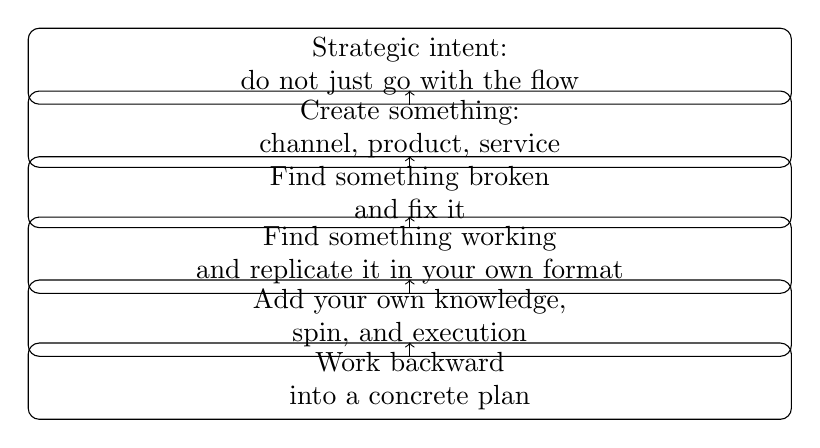
\begin{tikzpicture}[node distance=0.8cm]
\node[draw, rounded corners, align=center, text width=0.78\linewidth] (start) {Strategic intent:\\do not just go with the flow};
\node[draw, rounded corners, align=center, text width=0.78\linewidth, below of=start] (create) {Create something:\\channel, product, service};
\node[draw, rounded corners, align=center, text width=0.78\linewidth, below of=create] (fix) {Find something broken\\and fix it};
\node[draw, rounded corners, align=center, text width=0.78\linewidth, below of=fix] (replicate) {Find something working\\and replicate it in your own format};
\node[draw, rounded corners, align=center, text width=0.78\linewidth, below of=replicate] (spin) {Add your own knowledge,\\spin, and execution};
\node[draw, rounded corners, align=center, text width=0.78\linewidth, below of=spin] (plan) {Work backward\\into a concrete plan};
\draw[->] (start) -- (create);
\draw[->] (create) -- (fix);
\draw[->] (fix) -- (replicate);
\draw[->] (replicate) -- (spin);
\draw[->] (spin) -- (plan);
\end{tikzpicture}
\caption{Transcript-backed creation rule: create, fix, or replicate, then add differentiated execution and plan backward.}
\end{figure}

The next entrepreneur makes the risk more personal. He describes sitting in a Texas A\&M construction science classroom, already sensing the job path ahead, and deciding he had to jump. His junk removal company became a demolition company and then a land-clearing company. He says he started at \(21\), is \(28\), and has two other businesses.

His income claim is approximate:
\begin{equation}
I_{\mathrm{year}} \approx \$650{,}000.
\end{equation}
But he immediately adds volatility:
\begin{equation}
I_{\mathrm{month}} \in \{\$75{,}000,\ \$10{,}000,\ldots\}.
\end{equation}
This is one of the most important quantitative moments in the chapter. Annual income can look impressive while monthly income remains uneven. Entrepreneurship often trades salary smoothness for upside and variance.

When asked for his millionaire blueprint, he returns to real estate and planning. He recommends getting control of an appreciating asset early if possible, even with help from parents, then working backward from the desired end state. If he wants to build pools, he asks: what mechanical, electrical, plumbing, concrete, and specialty pieces are required? Who does them? Where are they? How good are they? The plan begins at the end and decomposes the path.

\section{Formal Credentials As Transferable Tools}

The final interviews widen the chapter from entrepreneurship alone to durable financial structures and transferable skill.

A retired law-enforcement professional says he spent about \(30\) years with the Los Angeles Police Department and at one point made more than \(300{,}000\) dollars doing celebrity weddings and security:
\begin{equation}
I_{\mathrm{year}} \gtrsim \$300{,}000.
\end{equation}
His financial advice is to invest. The transcript appears garbled around the phrase ``invest in diversity'' and ``pension in a divert,'' but the meaning is clear enough to state cautiously: he describes a pension plus a deferred compensation program, two buckets one can draw on later.

\begin{equation}
\hbox{retirement resources}
  =
  \hbox{pension}
  +
  \hbox{deferred compensation}.
\end{equation}
This is not a contribution formula. It is a structural lesson: do not depend on a single retirement source if another disciplined bucket is available.

The last speaker has an electrical engineering degree but works in cybersecurity and privacy. When asked about his best financial decision, he does not name a stock, a house, or a trade. He names engineering. Even if one does not work as an engineer, he says, the training opens different areas because it teaches problem solving.

That is the final turn of the lecture. The money question began as a number. It ends as a capability question. What do we own? What can we solve? What relationships can we sustain with real value? What structures do we build so that a single job or a single month does not determine the whole future?

\section{Summary}

The chapter's evidence is interview evidence, not blackboard mathematics. Still, the quantitative spine is clear. We distinguish personal income from revenue and profit. We separate cash from illiquid assets. We treat debt as capital plus obligation. We treat networking as access plus value. We treat annual income as a volatile output of a business system, not as a simple salary.

The recurring lesson is ownership under uncertainty. Some speakers own businesses, some own properties, some own relationships, some own skills, and some own disciplined retirement buckets. The income question starts the conversation, but the durable chapter is about the mechanisms that make income possible and the structures that keep it from disappearing.